\documentclass[french, a4paper, 12pt]{report}


\usepackage[frenchb]{babel}
\usepackage[utf8]{inputenc}
\usepackage[T1]{fontenc}
\usepackage{graphicx}
\usepackage{caption}
\usepackage{subcaption}
\setcounter{tocdepth}{3}
\setcounter{secnumdepth}{3}

\usepackage[frenchb]{babel}


\begin{document}


\chapter*{Remerciement}
\begin{center}
\Large \textbf{\textit{Tout d'abord, nous remercions Allah, notre créateur, pour nous avoir donné la force, la volonté et le courage d'accomplir ce modeste travail.\\
Nous remercions notre encadreur Monsieur Allaoui ansi que Madame Kerrouche pour leurs conseils et leur encouragement du début jusqu'à la fin de ce travail.\\
Nos remerciements vont aussi à tous ceux qui ont contribué de près ou de loin à la réalisation de ce travail.\\Enfin, nous tenons à exprimer notre profonde gratitude à nos familles qui nous ont toujours soutenus et à tous ceux qui ont participé à la réalisation de ce mémoire. Ainsi qu'à tous les enseignants qui ont contribué à notre formation.}}
\end{center}

\chapter*{Dédicaces}
\begin{center}
\Large \textbf{\textit{Nous dédions ce modeste travail à nos parents bien-aimés qui nous ont soutenus tout au long de notre cursus universitaire et le sont toujours.\\
À nos amis qui n'ont jamais hésité à nous aider de quelque manière que ce soit.\\
Et à tous ceux qui nous ont enseigné tout au long de notre vie scolaire.\\
A nos camarades de la 3ème année LMD.\\
Merci à tous.}}
\end{center}



\tableofcontents

\newpage
\addcontentsline{toc}{chapter}{Table des figures}
\listoffigures

\newpage
\addcontentsline{toc}{chapter}{Liste des tableaux}
\listoftables


\newpage
\chapter*{Liste des Abréviations}
\addcontentsline{toc}{chapter}{Liste des Abréviations}
	\begin{itemize}
		\item \textbf{MVC}:  Model View Controller
		\item \textbf{IHM}: Interface Homme Machine
		\item \textbf{SDK}: Software Development Kit
		\item \textbf{UML}: Unified Modeling Language
		\item \textbf{NoSQL}: Not only Structured Query Language
		\item \textbf{JSON}:  Java Script Object Notation
		\item \textbf{API}:  Application Programming Interface
	\end{itemize}


\newpage
\chapter*{Introduction}
    Au cours de la dernière décennie, nous avons assisté à une révolution dans les commerces en ligne. Les gens se sont habitués aux achats en ligne et aux réservations à distance comme la réservation de billets, l'achat d'articles et même la commande de nourriture, principalement parce que c'est plus rapide, sans effort et moins compliqué.\\\\

Lorsque quelqu'un veut acheter des repas en ligne, il doit chercher un restaurant qui prépare les repas désirés. La commande doit lui être livrée soit par le livreur du restaurant, soit par un établissement de livraison séparé.\\\\

Dans les pays étrangers, en Europe ou aux États-Unis, beaucoup de restaurants et de sociétés de livraison ont leur propre application mobile. Malheureusement, ce n'est pas le cas pour tous les établissements qui peuvent se permettre de créer leur propre application en raison des coûts élevés de développement d'une application mobile.\\\\

Delàs, nous avons pensé à contribuer à une solution. C'est une plateforme conçue comme une application mobile qui regroupe les clients, les restaurants et les établissements de livraison en un seul endroit. \\\\

Elle répond à tous les besoins des personnes qui veulent commander leurs plats à distance, elle permettra également aux propriétaires de restaurants et aux établissements de livraison d'augmenter leurs ventes et d'accélérer leur flux de travail avec les clients à distance.

\addcontentsline{toc}{chapter}{Introduction}

\newpage
\chapter{Receuil des besoins} Dans cette partie, nous proposons de regrouper les besoins techniques necessaires pour accomplir ce travail.
	\section{Développement Android} Nous avons choisi de réaliser une application mobile dédiée aux utilisateurs d'Android. Il existe beaucoup de choix quant aux technologies que nous allons utiliser pour ce développement.
		\subsection{Les technologies utilisées} Dans ce travail nous avons utilisé le framework Flutter pour les interfaces et la logique de l'application et Cloud Firestore de Firebase pour le stockage et la gestion de la base de données.
			\subsubsection*{Flutter} C'est un SDK d'interface utilisateur open-source créé par Google. Il est utilisé pour développer des applications multiplateformes pour Android, iOS, Linux, Mac, Windows et le Web à partir d'une base de code unique.\\Nous avons utilisé Flutter en raison de sa structure qui favorise la vitesse de développement. Sa structure est simplement une cascade de widgets faciles à personnaliser.

Flutter utilise le langage de programmation Dart, également développé par Google. Il s'agit d'un langage orienté objet, basé sur des classes avec une syntaxe de type de la language C.
			\subsubsection*{Firebase} C'est une plateforme accessible de n'importe quel endroit, qui aide à développer rapidement des applications de qualité. Elle dispose de nombreuses fonctionnalités, mais nous l'utilisons principalement pour son service de stockage au Cloud (Cloud Firestore).\\
				\paragraph*{Cloud Firestore} est une base de données documentaire NoSQL (un ensemble de continuation en cascade collection-document) qui nous permet de stocker, de synchroniser et d'interroger facilement des données pour des applications mobiles et web à l'échelle mondiale.
	\section{Méthode de travail collaborative}
		L'application conçue dans ce travail, a été développée à partir de zéro par trois développeurs. Nous avons travailler en parallèle sur le même projet, de ce fait nous, les trois développeurs, allons donc utiliser Git et Github.

		\subsection*{Git} C'est un logiciel permettant de suivre les modifications apportées à un ensemble de fichiers. Il est généralement utilisé pour coordonner le travail des programmeurs qui collaborent à l'élaboration du code source lors du développement de logiciels. Ses objectifs sont la rapidité, l'intégrité des données et la prise en charge des flux de travail distribués et non linéaires.

		\subsection*{Github} C'est un service d'hébergement de référentiel Git, mais il ajoute de nombreuses fonctionnalités qui lui sont propres. Il fournit une interface graphique basée sur le Web. Il fournit également un contrôle d'accès et plusieurs fonctions de collaboration.
	\section{Architecture du code} %include the sequence chart of flutter in mvc
		Nous avons utilisé l'architecture de projet MVC. Il s'agit d'un modèle de conception de logiciel couramment utilisé pour développer des interfaces utilisateur qui divisent la logique du programme en trois éléments interconnectés.

Cela permet de séparer les représentations internes de l'information de la manière dont l'information est présentée à l'utilisateur et acceptée par celui-ci.
\begin{figure}[!h]
  \center
  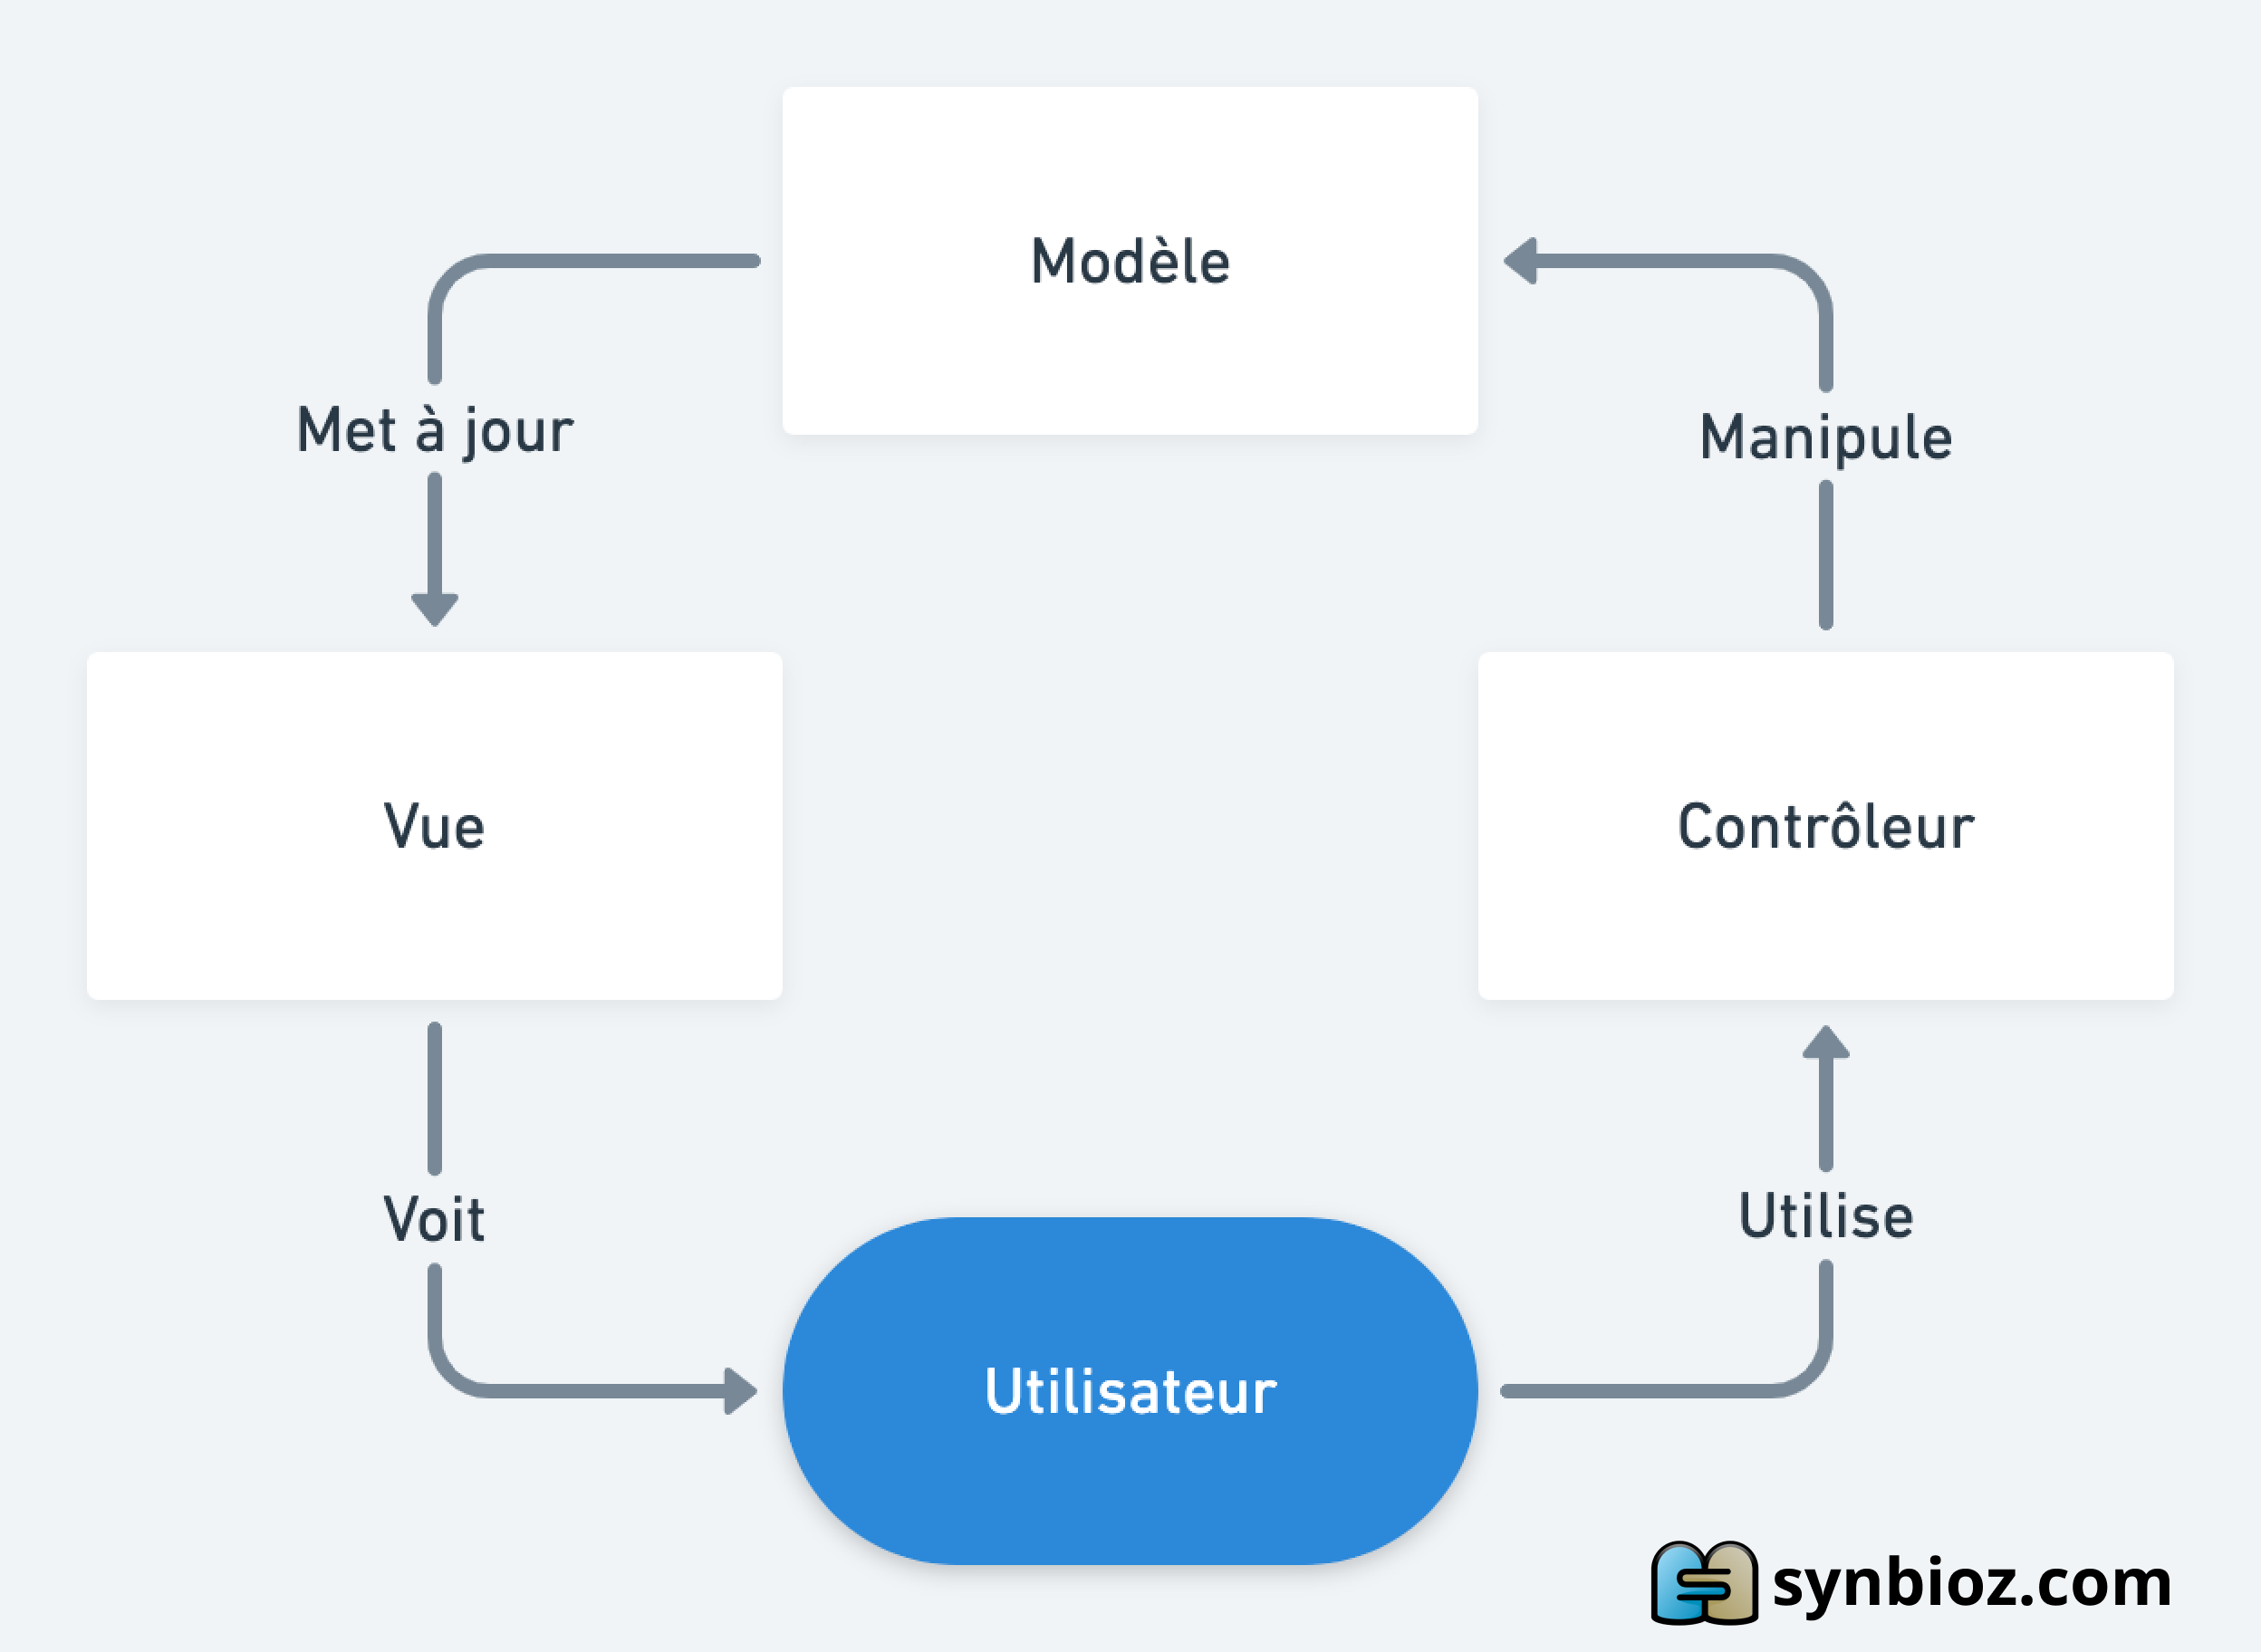
\includegraphics[width=10cm]{mvc.png}
  \caption{Le flux MVC}
  \label{fig:fluxmvc}
\end{figure}

\newpage
\chapter{Conception de l'application} Dans ce chapitre nous présentons les differentes étapes de la conception de l'application de gestion de commande et livraison de la restauration.
	\section{Modélisation} On a choisi trois diagrammes d’UML pour modéliser l'application:
		\begin{itemize}
			\item Diagramme de classes
			\item Diagrammes de cas d’utilisation
			\item Diagrammes de séquence
		\end{itemize}
		
		\newpage
		\subsubsection{Diagramme de classes}
			\begin{figure}[!h]
  				\center
  				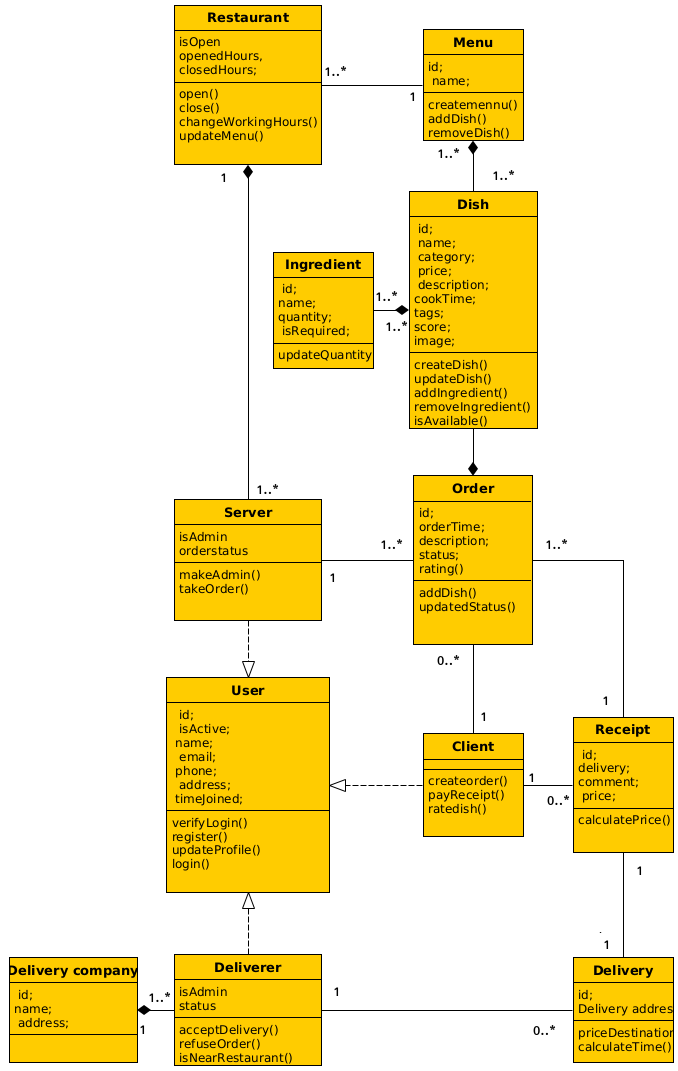
\includegraphics[width=10cm]{classdiag.png}
  				\caption{Diagramme de classes}
  				\label{fig:classdiag}
			\end{figure}
			
			La figure (fig \ref{fig:classdiag}) décrit les classes principales d'objets sur lesquelles repose la logique de l'application, ainsi que les relations qui existent entre elles.
			\newpage
			Le tableau (tab \ref{tab:classdiag}) explique le schéma de figure \ref{fig:classdiag}, dans lequel les classes sont définies comme suit:
			
			\begin{table}[!h!]
  				\begin{tabular}{lllp{6cm}}
    					Classes & Attributs & Méthodes & Relations \\ 

					\hline
    					Delivery company & & & Elle a un ou plusieurs livreurs \\  
    					
    					\hline
    					Restaurant & & & Il a un ou plusieurs serveurs et un menu \\   					
    					
    					\hline
    					User & & & Le Client et le Serveur et le Livreur héritent de ses attributs et de ses méthodes \\
    					
					\hline
    					Client & & & Il peut avoir des commandes et des recettes multiples\\  
    					  					
    					\hline
    					Server & & & Il appartient à un restaurant et peut avoir plusieurs commandes \\
    					
    					\hline
    					Deliverer & & & Il appartient à une société de livraison et peut avoir plusieurs livraisons \\
    					    					
    					\hline
    					Menu & & & Il peut appartenir à plusieurs restaurants et avoir plus d'un plat\\
    					
    					\hline
					Dish & & & Il appartient à un ou plusieurs menus et comporte plusieurs ingrédients \\

						
					\hline
					Ingredient & & & Il appartient à un ou plusieurs plats \\
						
					\hline
					Order & & & Il appartient à un serveur et à un client, et à un reçu \\
						
					\hline
					Delivery & & & Elle appartient à un livreur et à un reçu \\
						
					\hline	
					Receipt & & & Il appartient à un client \\
    					
  				\end{tabular}
  				\caption{Déconstruction du diagramme de classe}
  				\label{tab:classdiag}
			\end{table}

		\newpage
		\subsubsection{Diagrammes de cas d’utilisation} Dans cette section, nous présentons les diagrammes de cas d'utilisation. Nous avons réalisé un diagramme pour les principales utilisations qui se déroulent dans l'application. 
		
		%\newpage	
			
			\begin{figure}[!h]
  				\center
  				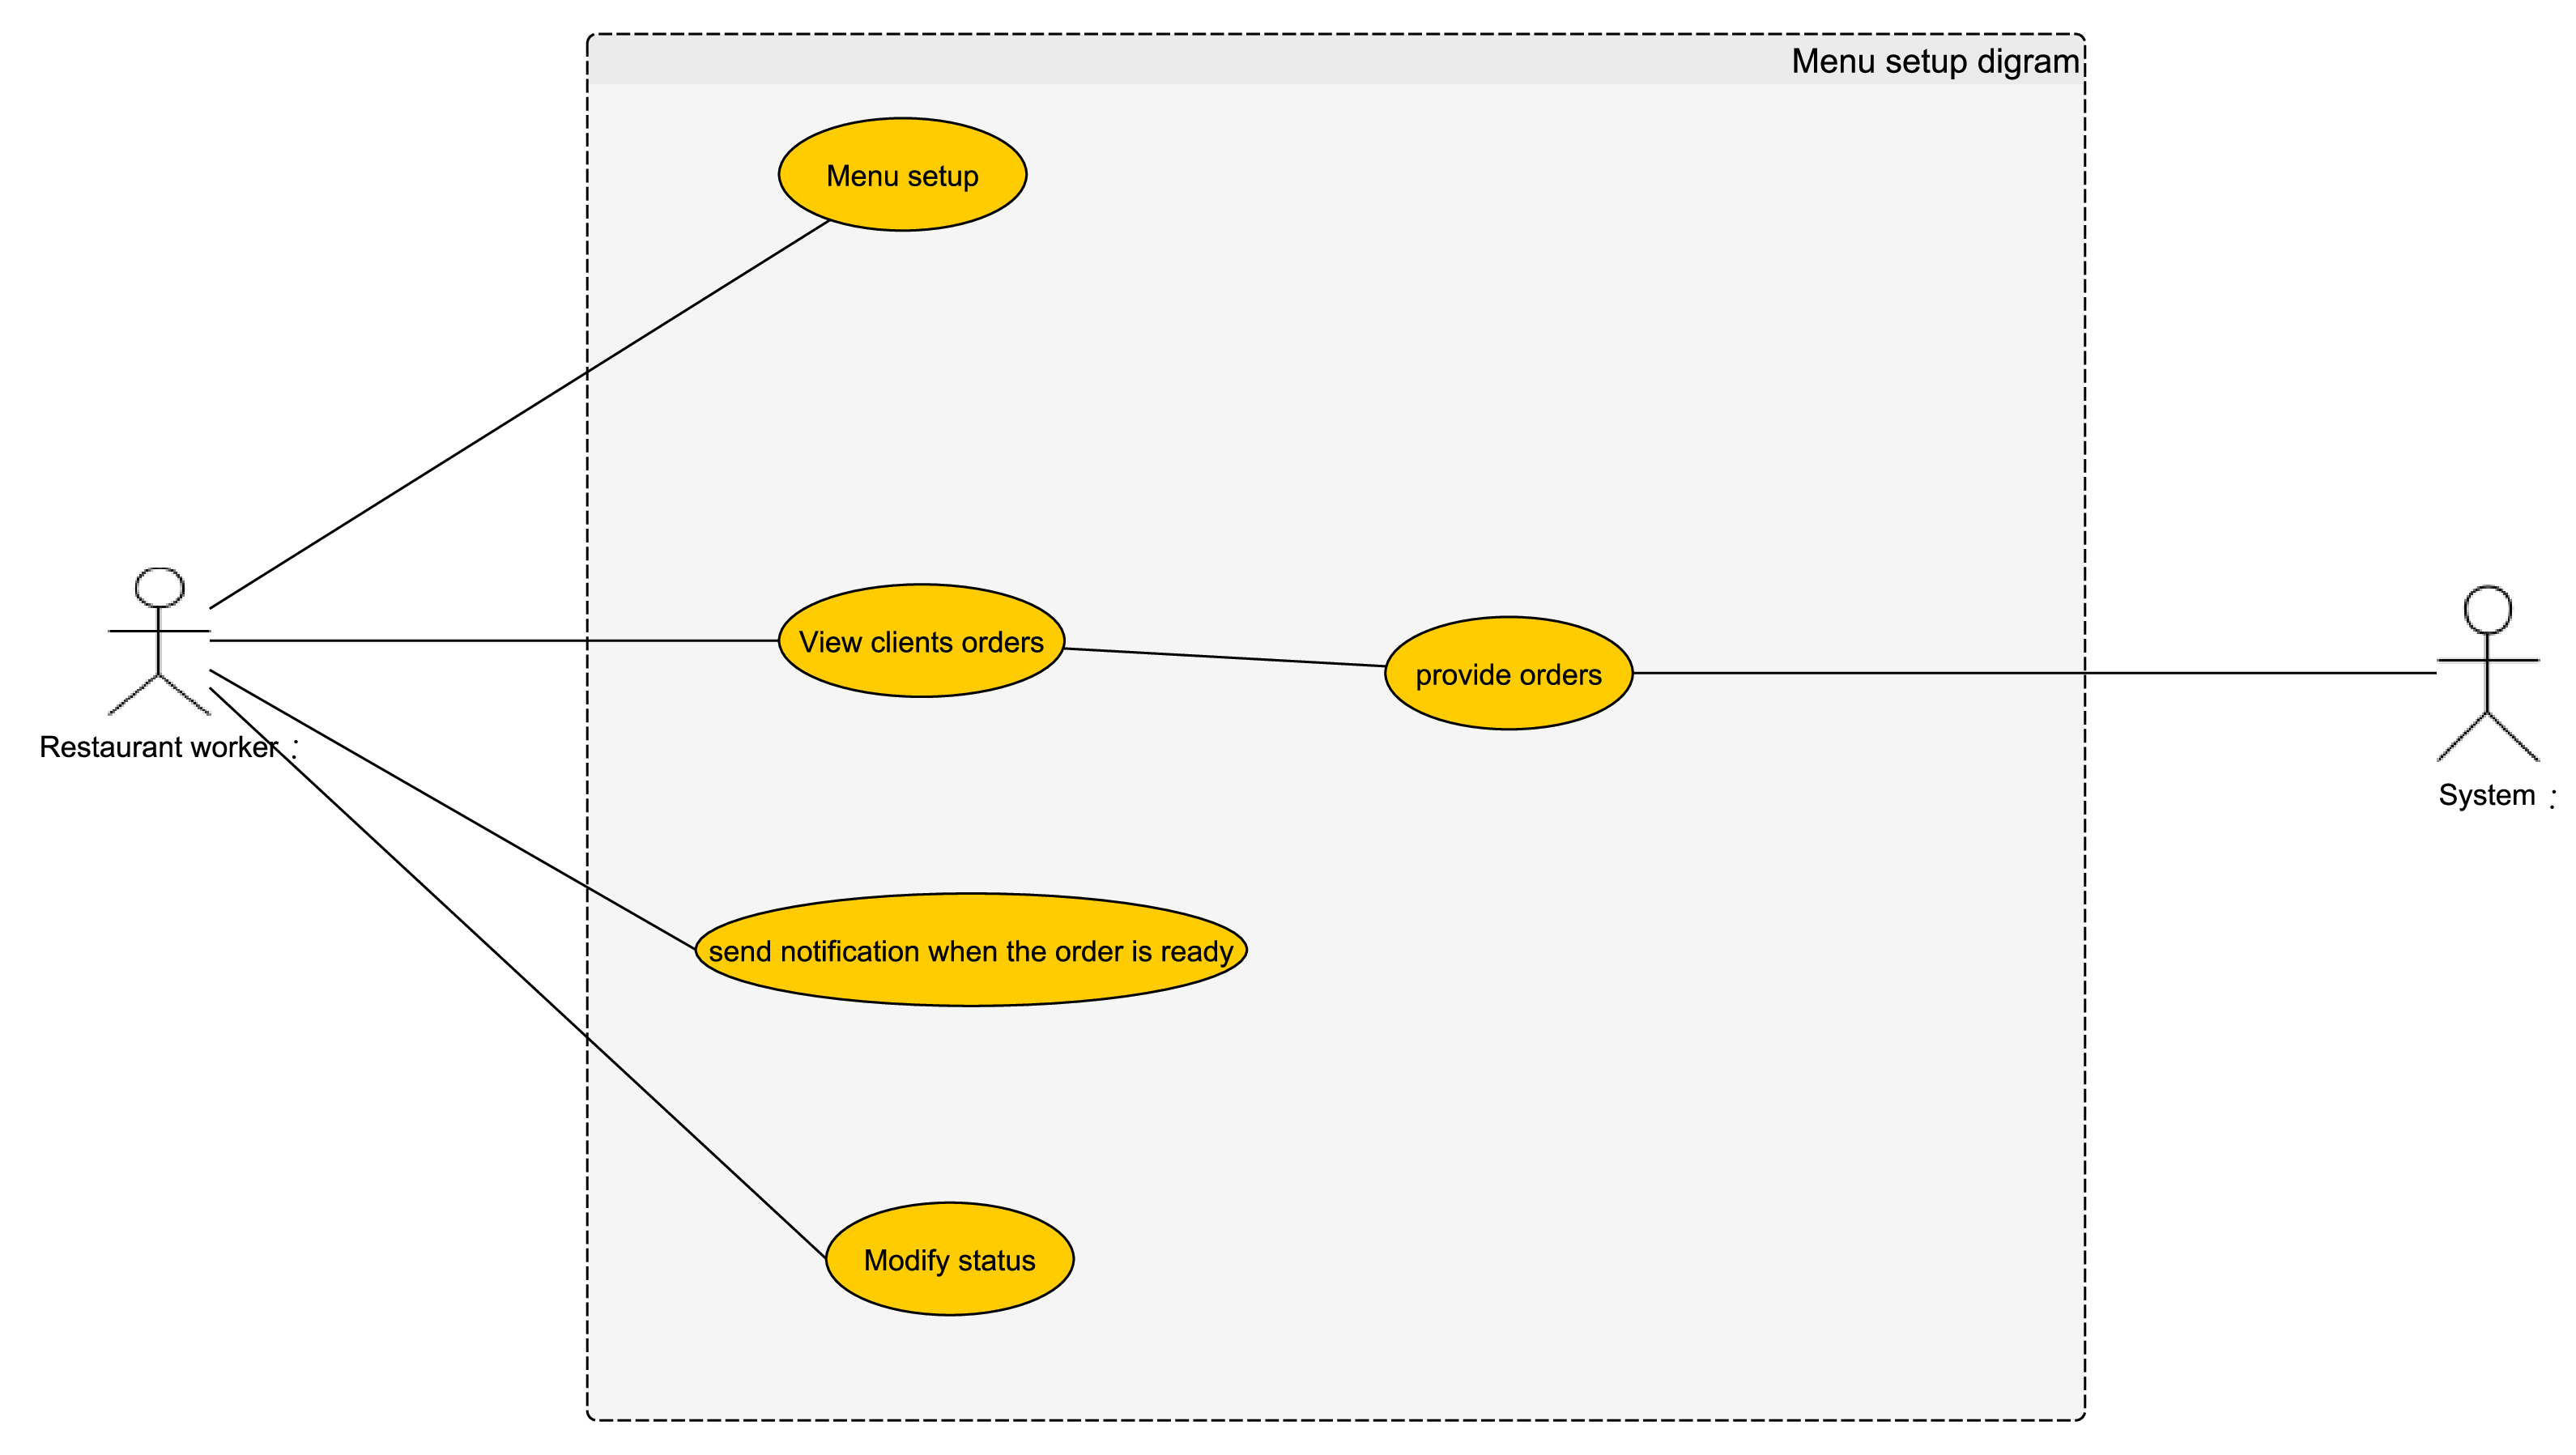
\includegraphics[width=15cm]{usecasemenu.png}
  				\caption{Diagramme de cas d'ustilisation du configuration du menu}
  				\label{fig:usecasemenu}
			\end{figure}
			
			La figure (fig \ref{fig:usecasemenu}) illustre le cas de la configuration du menu du restaurant par l'employé du restaurant. L'employé du restaurant (serveur) a la possibilité de contrôler
le menu (ajouter, modifier et supprimer des plats), et recevoir les commandes du client que le système lui fournit,
il a aussi le contrôle total de l'état de chaque commande (en préparation, ou prête à être livrée).
			
			\newpage
			\begin{figure}[!h]
  				\center
  				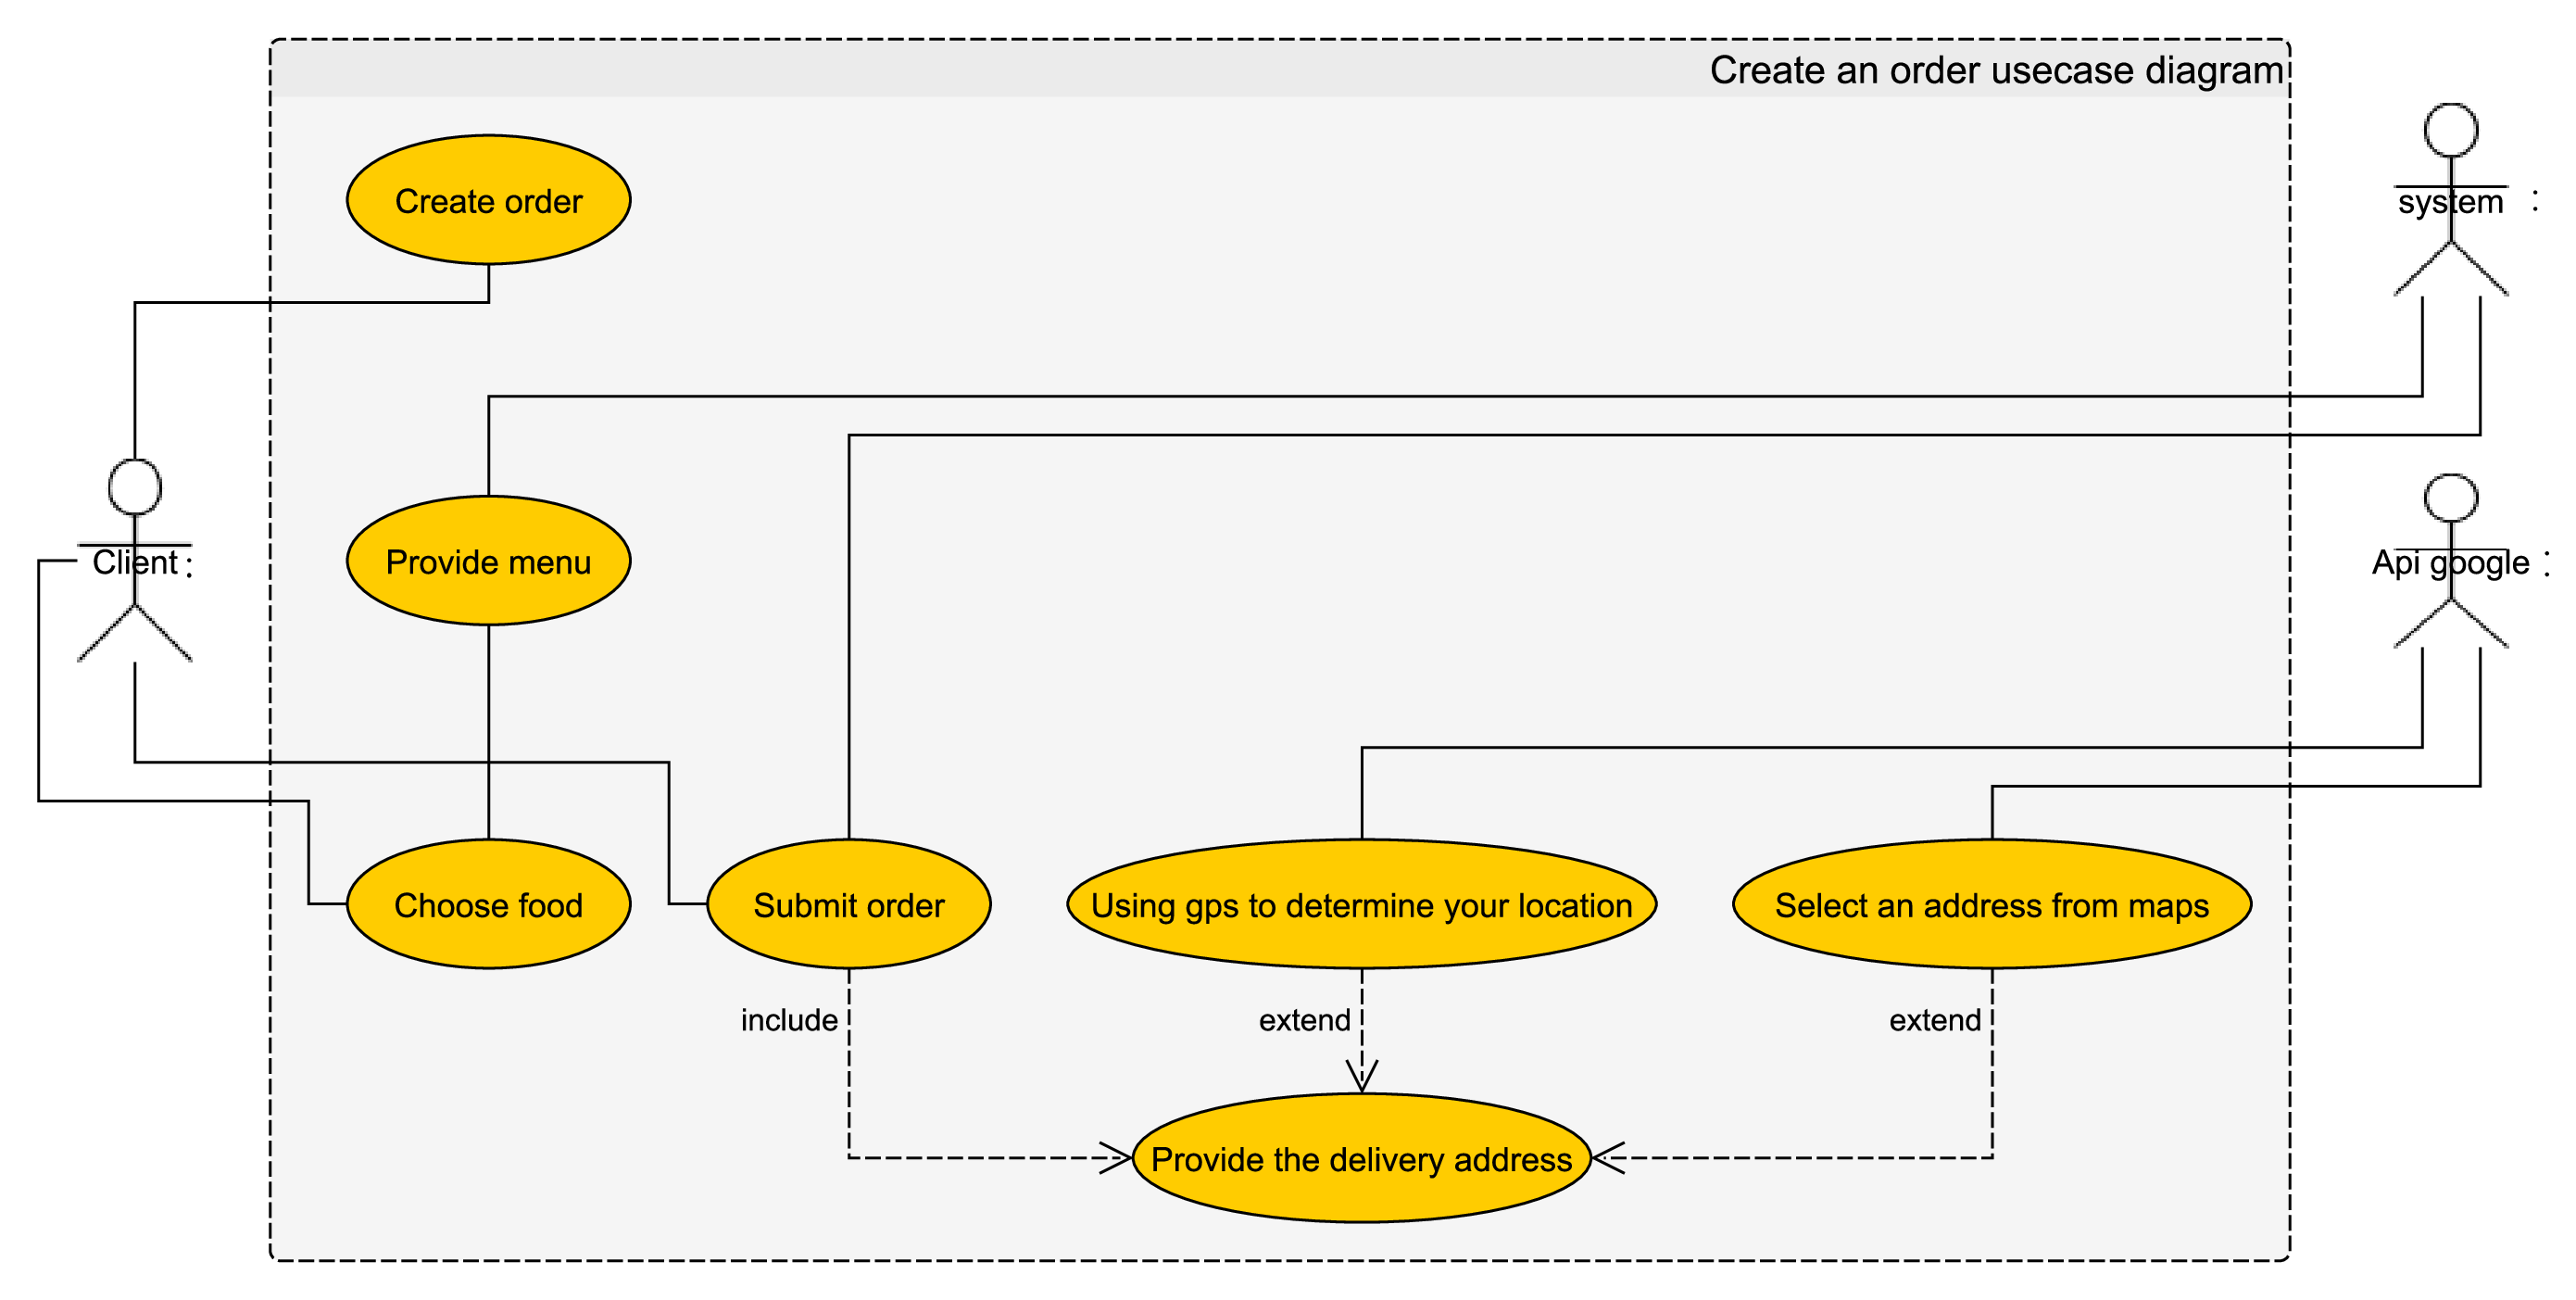
\includegraphics[width=15cm]{usecaseorder.png}
  				\caption{Diagramme de cas d'ustilisation de passation d'une commande}
  				\label{fig:usecaseorder}
			\end{figure}
			La figure (fig \ref{fig:usecaseorder}) illustre le cas de la configuration de passation d'une commande par le client de restaurant. Le système met à disposition aux clients des restaurants et leurs menus afin que le client puisse choisir son restaurant,
puis choisir ses plats. Il confirme ensuite la commande en indiquant l'adresse de livraison et les informations nécessaires. La commande est soumise au système pour être traitée.
			
			\newpage
			\begin{figure}[!h]
  				\center
  				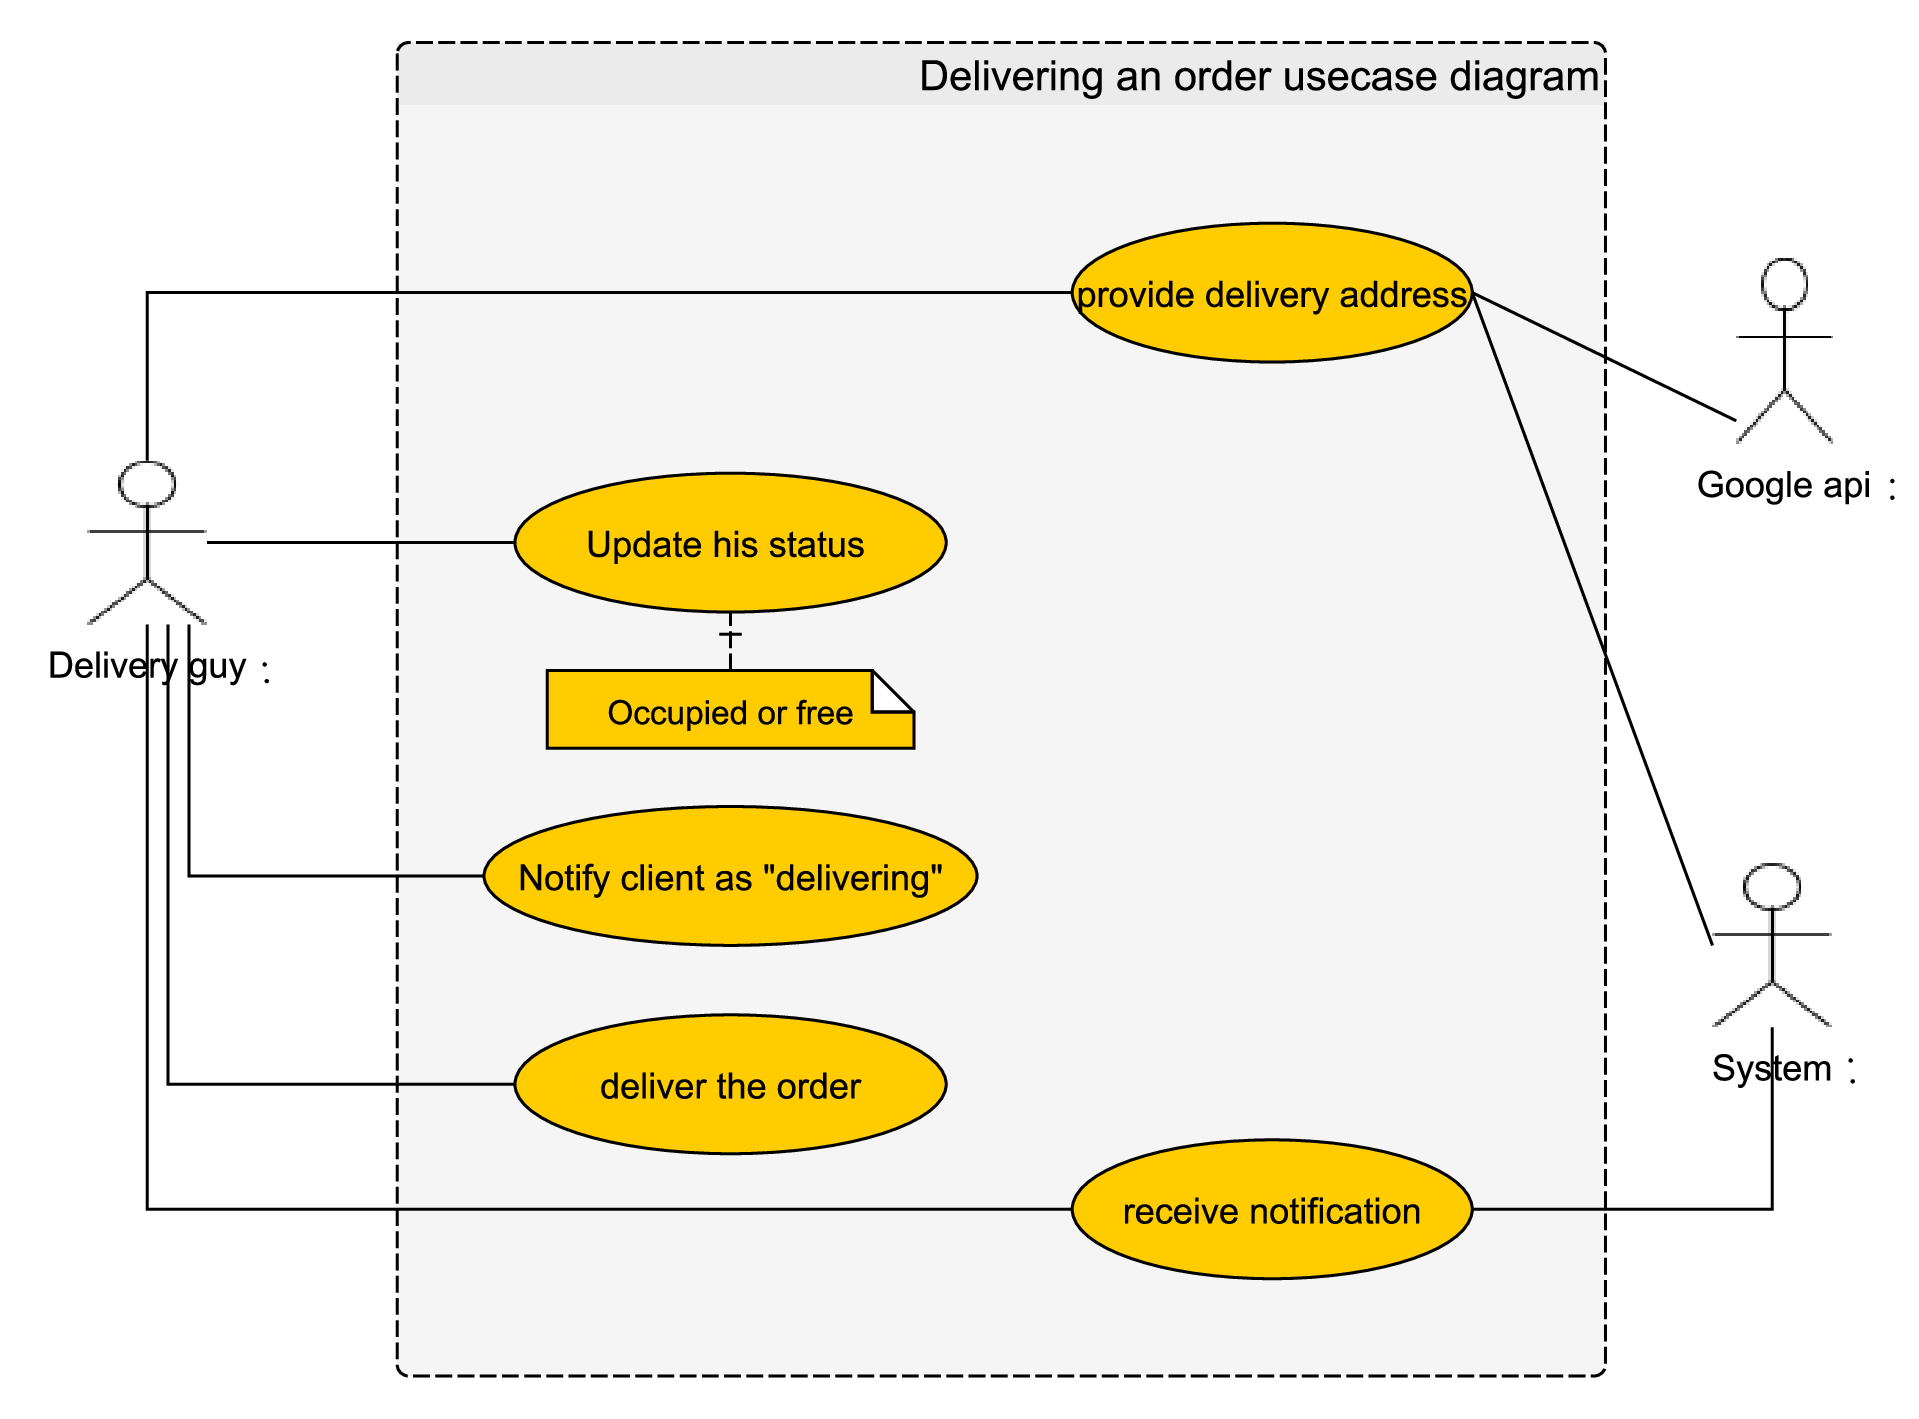
\includegraphics[width=15cm]{usecasedeliver.png}
  				\caption{Diagramme de cas d'ustilisation du livraison d'une commande}
  				\label{fig:usecasedeliver}
			\end{figure}
			La figure (fig \ref{fig:usecasedeliver}) illustre le cas de la livraison d'une commande par le livreur. Les livreurs ont la possibilité de définir leur statut "occupé" ou "libre". Lorsqu'un livreur proche accepte une livraison de sa liste de livraisons proches (commandes prêtes à être livrées), il a alors accès à toutes les informations nécessaires de l'adresse du restaurant et de l'adresse du client.
Chaque livreur a la possibilité d'informer le client de l'état de livraison de la commande.
			
			
			\newpage
		\subsubsection{Diagrammes de séquences} Dans cette section, nous allons illustrer les séquences d'interactions entre les utilisateurs et le système à l'aide des diagrammes de séquence d'UML.
			\begin{figure}[h!]
  				\center
  				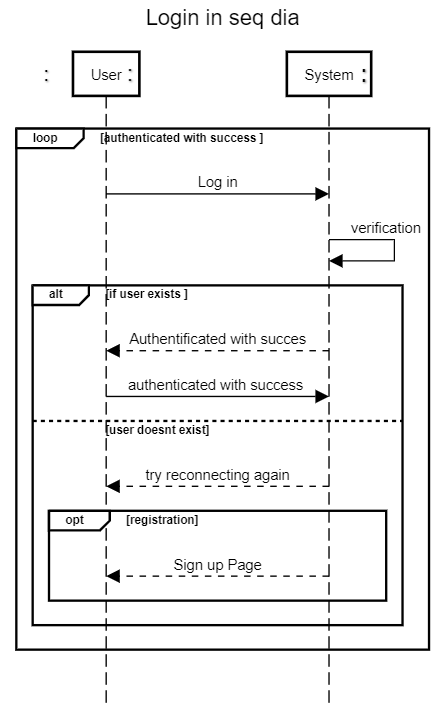
\includegraphics[width=10cm]{seqlogin.png}
  				\caption{Diagramme de séquences du authentification}
  				\label{fig:seqlogin}
			\end{figure} \\La figure (fig \ref{fig:seqlogin}) décrit la séquence de connexion au système par tout utilisateur. L'utilisateur saisit ses informations d'identification, le système vérifie si l'utilisateur existe. S'il existe, le système authentifie sa connexion avec succès, sinon il donne à l'utilisateur la possibilité de s'inscrire ou de saisir à nouveau ses informations d'identification. L'ensemble du processus se répète jusqu'à ce que l'utilisateur se connecte avec succès.
			
			\newpage	
			\begin{figure}[!h]
  				\center
  				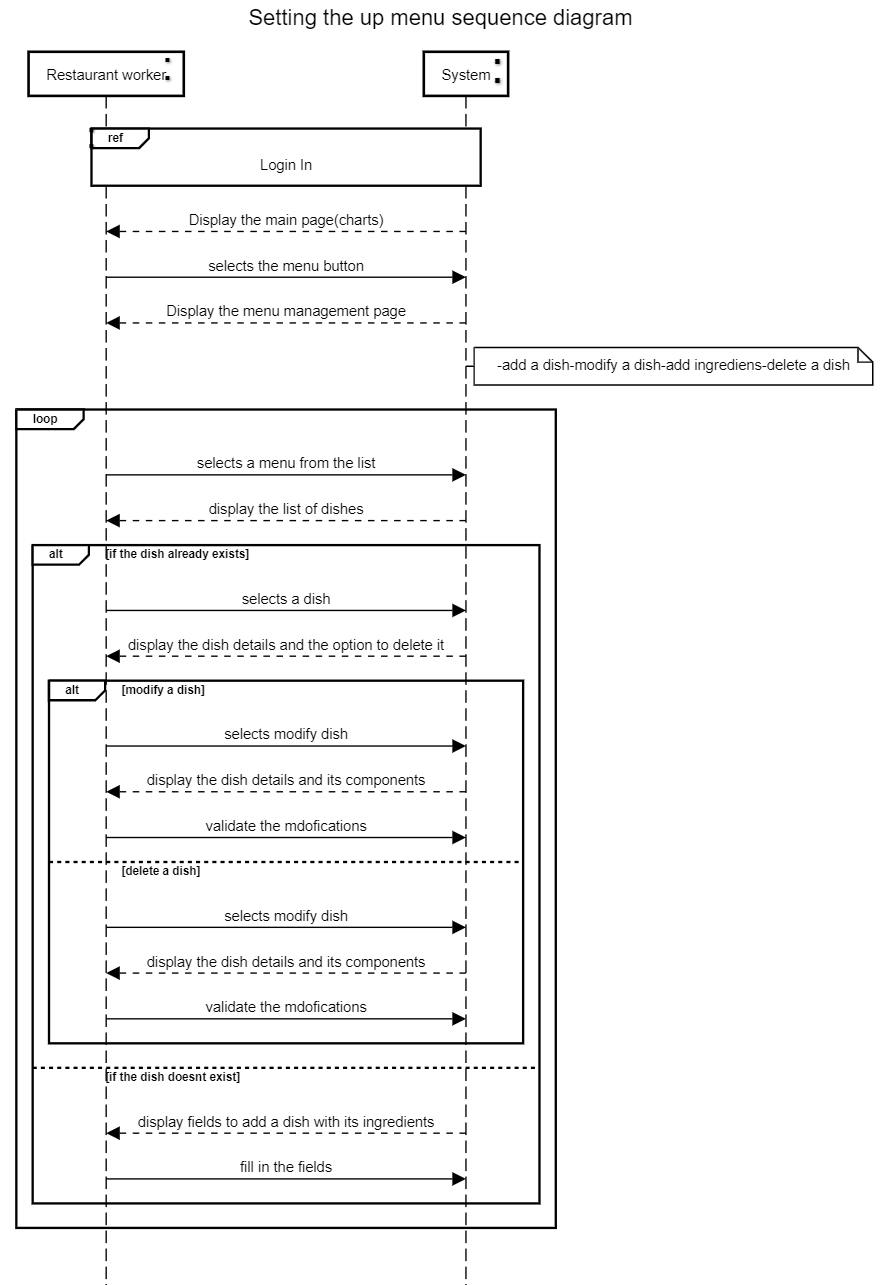
\includegraphics[width=12cm]{seqmenu.png}
  				\caption{Diagramme de séquences du configuration du menu}
  				\label{fig:seqmenu}
			\end{figure} La figure (fig \ref{fig:seqmenu}) décrit la séquence de configuration de menu du restaurant. Après que l'employé du restaurant se soit connecté avec succès, il peut choisir d'accéder à la page de gestion du menu dans laquelle il peut sélectionner un plat dans une liste de plats s'ils existent déjà dans le menu pour les supprimer ou les modifier. S'il choisit de les modifier, le système lui montrera tous les détails du plat à modifier, puis après la modification, il pourra valider ses changements. Si le menu est vide, le système fournira un formulaire pour remplir toutes les informations sur le plat avec ses ingrédients.
			
			\newpage	
			\begin{figure}[!h]
  				\center
  				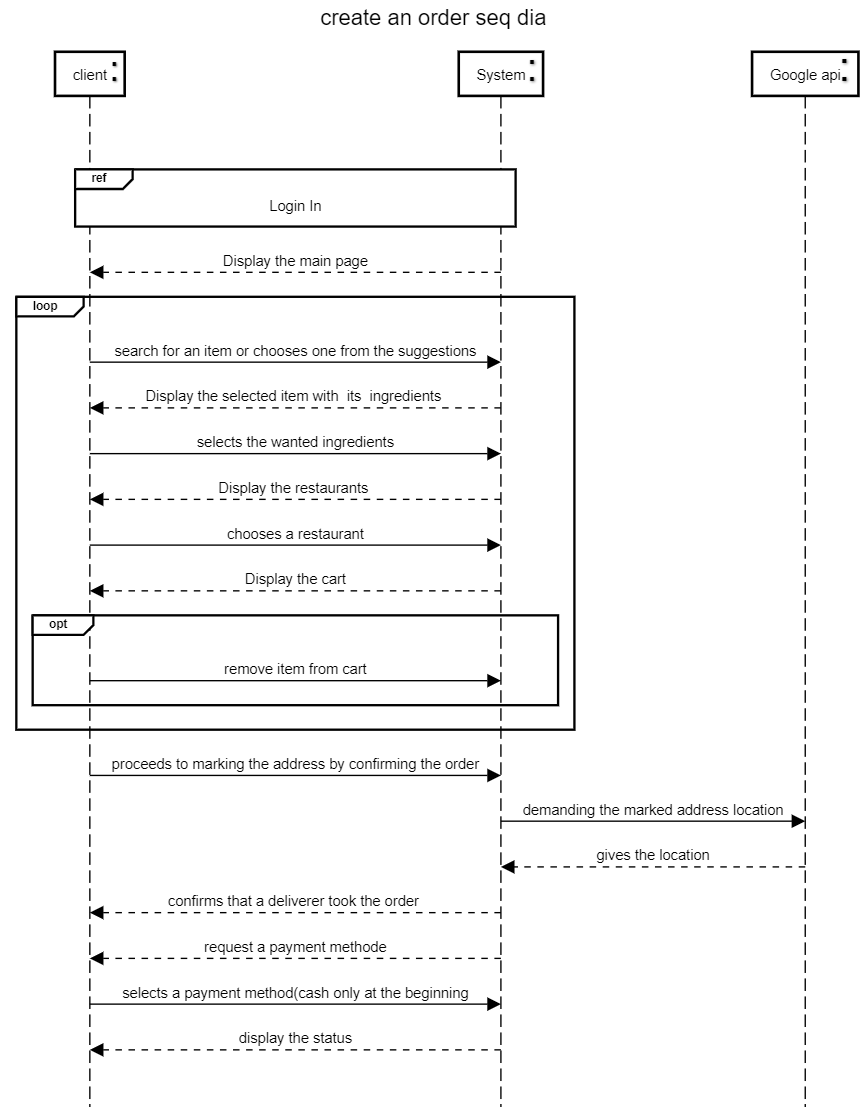
\includegraphics[width=15cm]{seqorder.png}
  				\caption{Diagramme de séquences de passation d'une commande}
  				\label{fig:seqorder}
			\end{figure} La figure (fig \ref{fig:seqorder}) décrit la séquence de passation d'une commande par le client. Une fois que le client a réussi à se connecter, le système lui montre la page principale.\\Le client peut rechercher un plat spécifique ou sélectionner un restaurant, puis sélectionner le plat, le système affichera le plat dans lequel le client peut sélectionner les ingrédients souhaités, puis ajouter le plat au panier.\\Il peut répéter ce processus jusqu'à ce que tous les plats qu'il souhaite soient ajoutés au panier (il a également la possibilité de retirer un plat du panier).\\\\
Le client peut ensuite procéder au marquage de l'adresse de livraison sur la carte, le système obtiendra les détails de l'emplacement à partir de l'API Google Maps.\\
Le système demandera une option de paiement, et après validation, le système mettra à jour l'état de la commande en la mettant en "attente" jusqu'à ce que l'employé du restaurant commence à la préparer.
			
			\newpage	
			\begin{figure}[!h]
  				\center
  				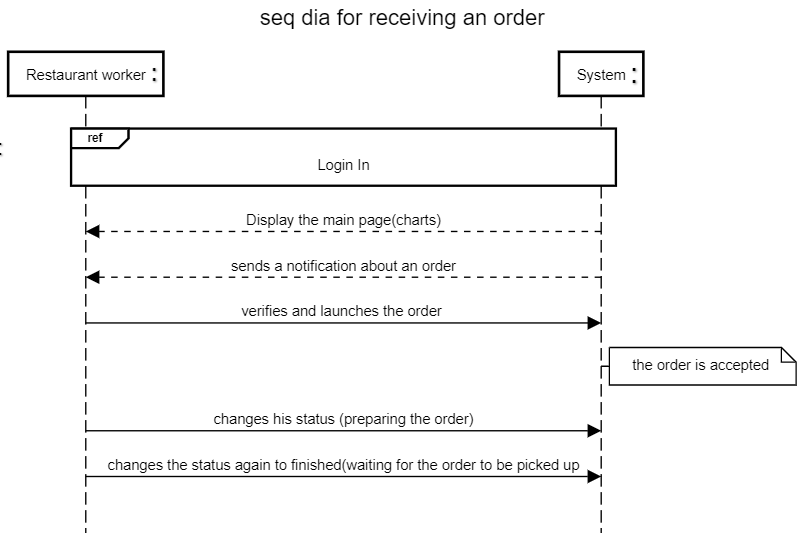
\includegraphics[width=12cm]{seqrest.png}
  				\caption{Diagramme de séquences du recepetion d'une commande}
  				\label{fig:seqrest}
			\end{figure} La figure (fig \ref{fig:seqrest}) décrit la séquence du recepetion d'une commande par l'employé du restaurant (serveur). Lorsqu'une commande est passée, l'employé du restaurant est notifié par le système. Le serveur valide la commande et commence à la préparer. Le système notifie alors au client le changement de statut de la commande, qui passe de "en attente" à "en préparation".
Une fois la commande prête, le serveur met à jour le statut de la commande en "prêt à livrer".
			
			\newpage	
			\begin{figure}[!h]
  				\center
  				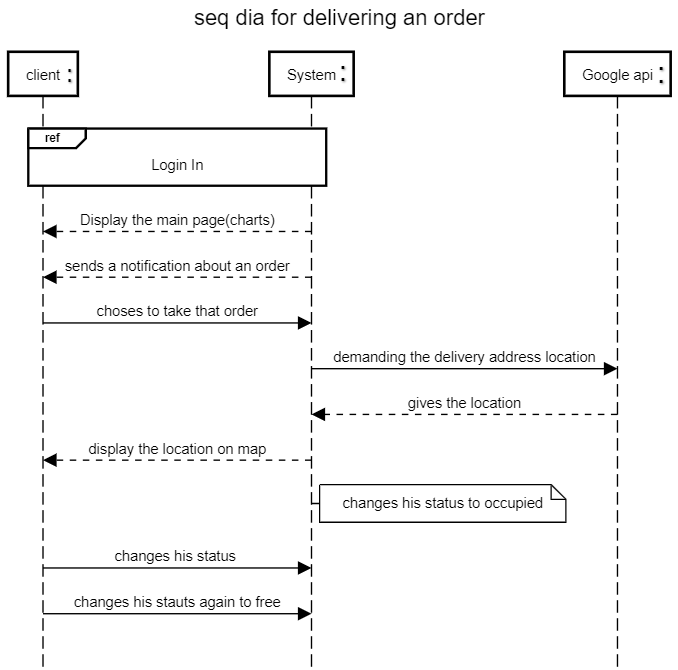
\includegraphics[width=10cm]{seqdeliver.png}
  				\caption{Diagramme de séquences du livraison d'une commande}
  				\label{fig:seqdeliver}
			\end{figure} La figure (fig \ref{fig:seqdeliver}) décrit la séquence du livraison d'une commande. Si le statut d'une commande est défini comme "prêt à être livré", le livreur en est informé par le système.
Lorsqu'il décide d'accepter la livraison, le système lui envoie toutes les informations nécessaires sur les lieux de départ et d'arrivée.
Le livreur peut changer le statut de la commande en "livraison" une fois qu'il l'a récupérée au restaurant.
Après la livraison, il peut changer son statut de "occupé" à "libre".


	
	\newpage		
	\section{La structure du code}
		\subsection{Modéles} Nous avons représenté chaque classe du diagramme de classes (Fig. \ref{fig:classdiag}) comme des classes Dart pour les traiter comme des objets. Chacune de ces classes possède deux méthodes permettant de convertir de et vers des objets JSON  pour faciliter la communication avec la base de données.
		\subsection{Contrôleurs} Ils représentent la fonctionnalité principale de chaque action dans l'application, de la connexion à la mise à jour des commandes et tout ce qui est similaire.
		\subsection{Vues} Chaque écran qui apparaît à l'utilisateur est considéré comme une vue. Les vues contiennent plusieurs widgets en cascade.
		\subsection{Widgets} Nous avons dû créer des widgets personnalisés pour répondre à nos besoins, comme des boutons, des vues de liste, des vues de texte, etc.
		
\newpage
\chapter{Réalisation de l'application} Dans ce chapitre nous allons présenter les differentes IHMs de flux de cette application.
	\section{Lancement d'application} Lorsque l'application est lancée pour la première fois, elle affiche la page de connexion (fig. \ref{fig:signin}).
Lorsqu'un nouvel utilisateur souhaite accéder à l'application, il doit d'abord s'inscrire en cliquant sur le bouton "Sign up".

\begin{figure}[h!]
\centering
\begin{subfigure}{.5\textwidth}
  \centering
  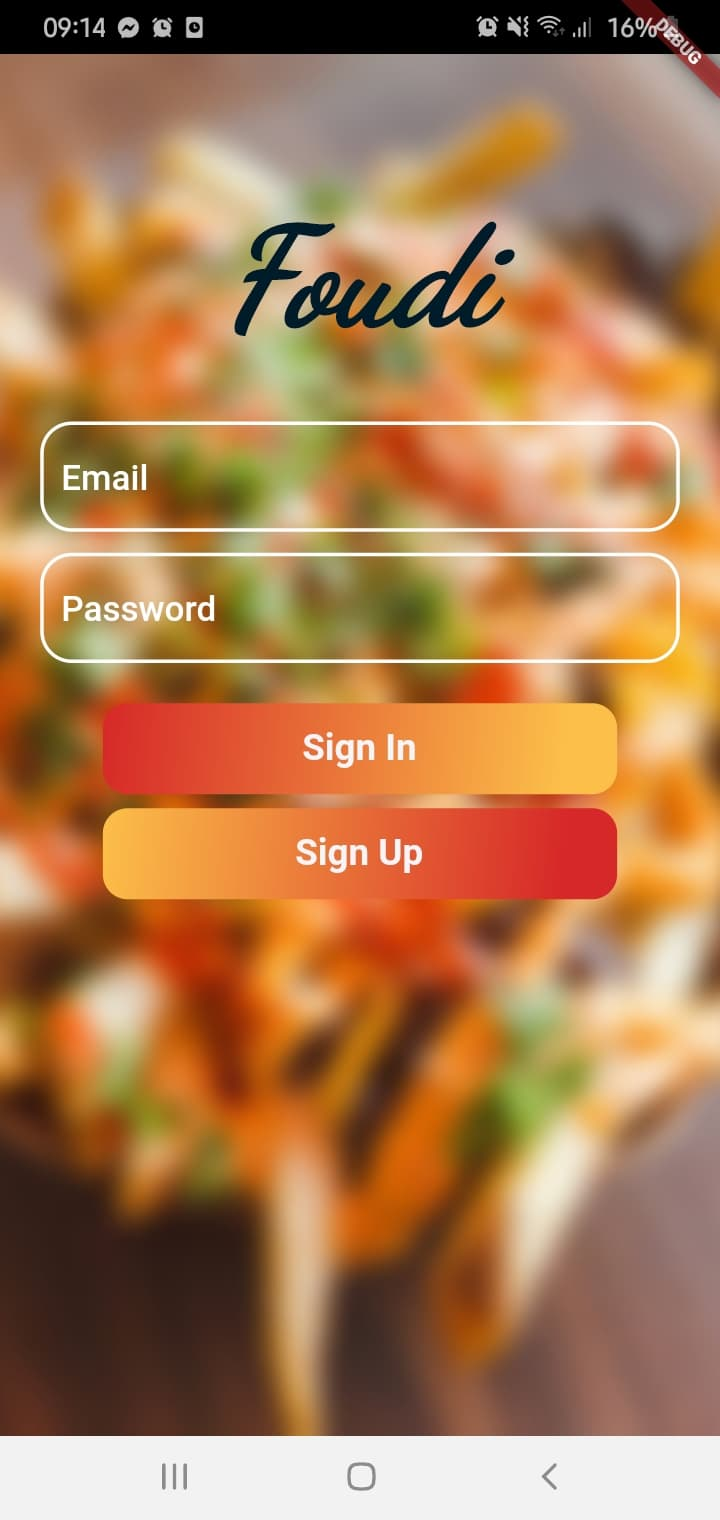
\includegraphics[width=.9\linewidth]{screenshots/signin.jpg}
  \caption{L'IHM de la page de connexion}
  \label{fig:signin}
\end{subfigure}%
\begin{subfigure}{.5\textwidth}
  \centering
  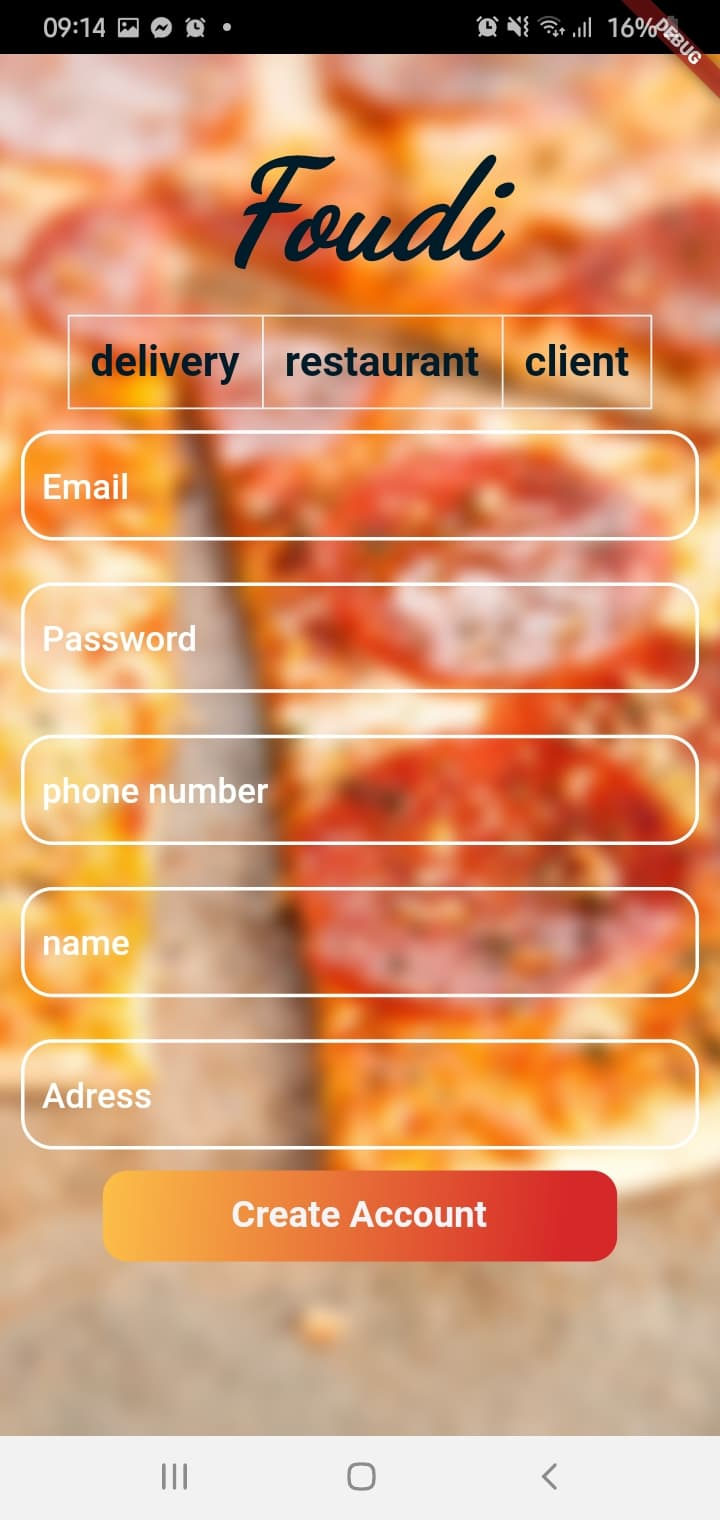
\includegraphics[width=.9\linewidth]{screenshots/signup.jpg}
  \caption{L'IHM de la page d'inscription}
  \label{fig:signup}
\end{subfigure}
\caption{A figure with two subfigures}
\label{fig:lanc}
\end{figure}
		
		\subsubsection{L'inscription} Comme la figure (fig \ref{fig:signup}) le montre, le nouvel utilisateur doit choisir le type de compte (Client, Restaurant, ou Delivery). Il remplit ensuite les informations nécessaires et appuie sur "Create Account".
Le système vérifiera si l'utilisateur n'existe pas déjà et validera ensuite son compte.	
		\subsubsection{La connexion (Login)} Si l'utilisateur possède déjà un compte, il peut saisir son e-mail et son mot de passe (comme en fig. \ref{fig:signin}). Le système détectera automatiquement le type d'utilisateur et lui montrera sa page d'accueil qui lui correspond.
		 
	\newpage
	\section{Cas d'utilisateur client} *flux*
	\newpage
	\section{Cas d'utilisateur server} Le server (employé du restaurant) dispose de trois pages dans le menu de l'application:
		\begin{itemize}
			\item \textbf{Page des commandes (page d'accueil)}: Une liste de toutes les commandes passées
			\item \textbf{Page de configuration du menu}: Pour modifier le menu du restaurant
			\item \textbf{Page de profile}: Pour voir les avis des client vis à vis de son restaurant.
		\end{itemize}
		
		\subsection{La page des commandes}
		
		\begin{figure}[h!]
			\center
			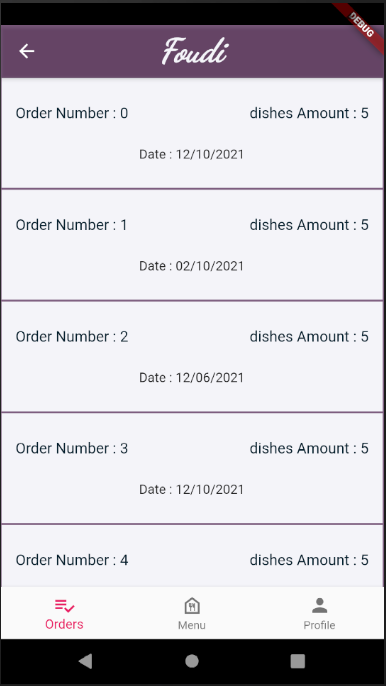
\includegraphics[width=5cm]{screenshots/Restaurantviews/ListofOrders(received).png}
			\caption{L'IHM de la page des commandes}
			\label{fig:restord}	
		\end{figure} Le système fournit au travailleur du restaurant les commandes des clients (fig \ref{fig:restord}), chaque commande contient (lorsqu'il est pressé) les informations nécessaires (un identifiant et une heure de commande, des plats avec les ingrédients souhaités, des notes si disponibles...etc) comme c'est indiqué dans  la figure (fig \ref{fig:restdish}).
		
		\newpage
		\begin{figure}[h!]
			\center
			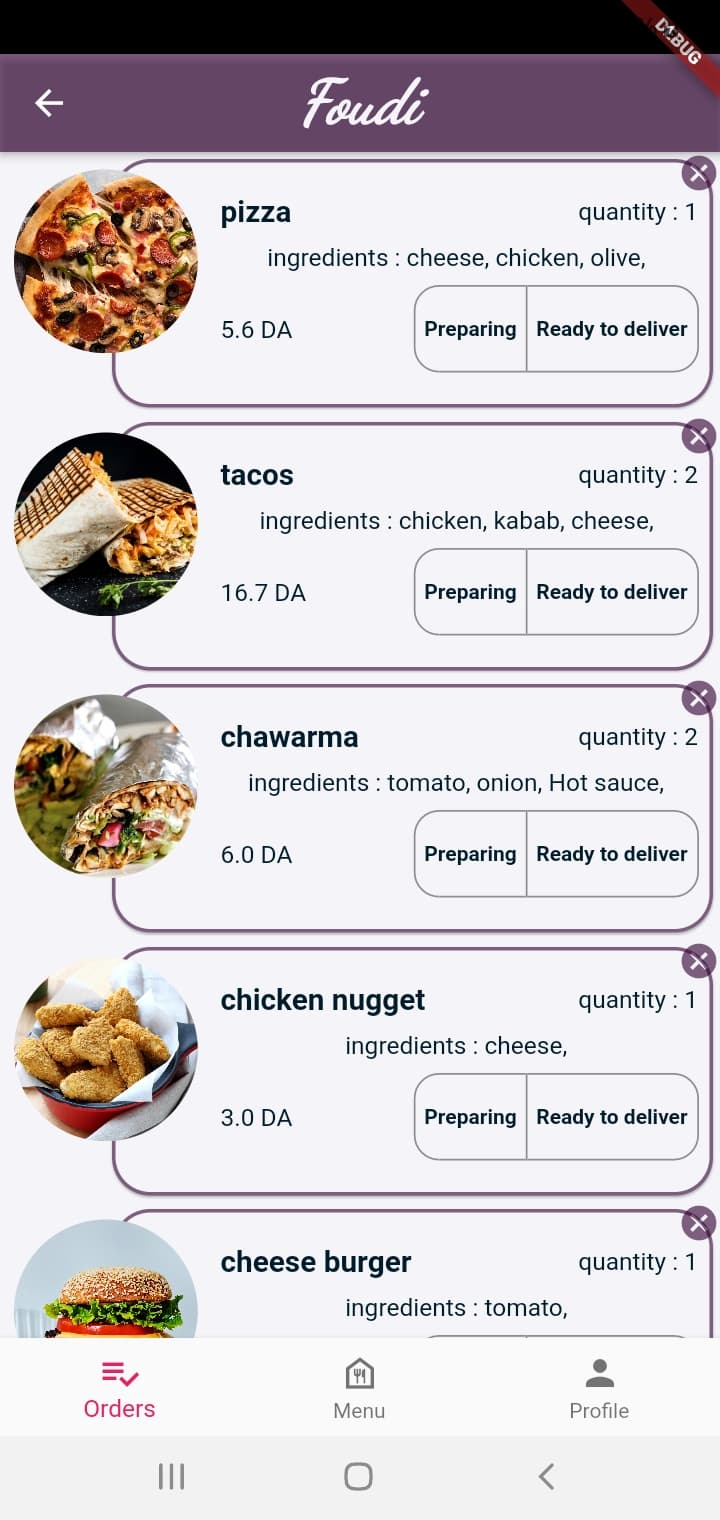
\includegraphics[width=5cm]{screenshots/Restaurantviews/ListofDishes.jpg}
			\caption{L'IHM de la page plats dans un commande}
			\label{fig:restdish}	
		\end{figure}
		Lorsque la commande commence à être préparée, le serveur met l'état de la commande en préparation pour en informer le client. Après avoir terminé, il met l'état de la commande sur prêt à livrer pour que le livreur soit notifié.
		
		\subsection{La page de configuration du menu} L'employé du restaurant a la possibilité d'ajouter et de supprimer des plats du menu du restaurant (fig \ref{fig:restconfig}), ainsi que la possibilité de modifier les ingrédients en les activant ou en les désactivant simplement en cliquant sur un simple bouton à bascule (fig \ref{fig:restedit}).
		
		\newpage

\begin{figure}[h!]
\centering
\begin{subfigure}{.5\textwidth}
  \centering
  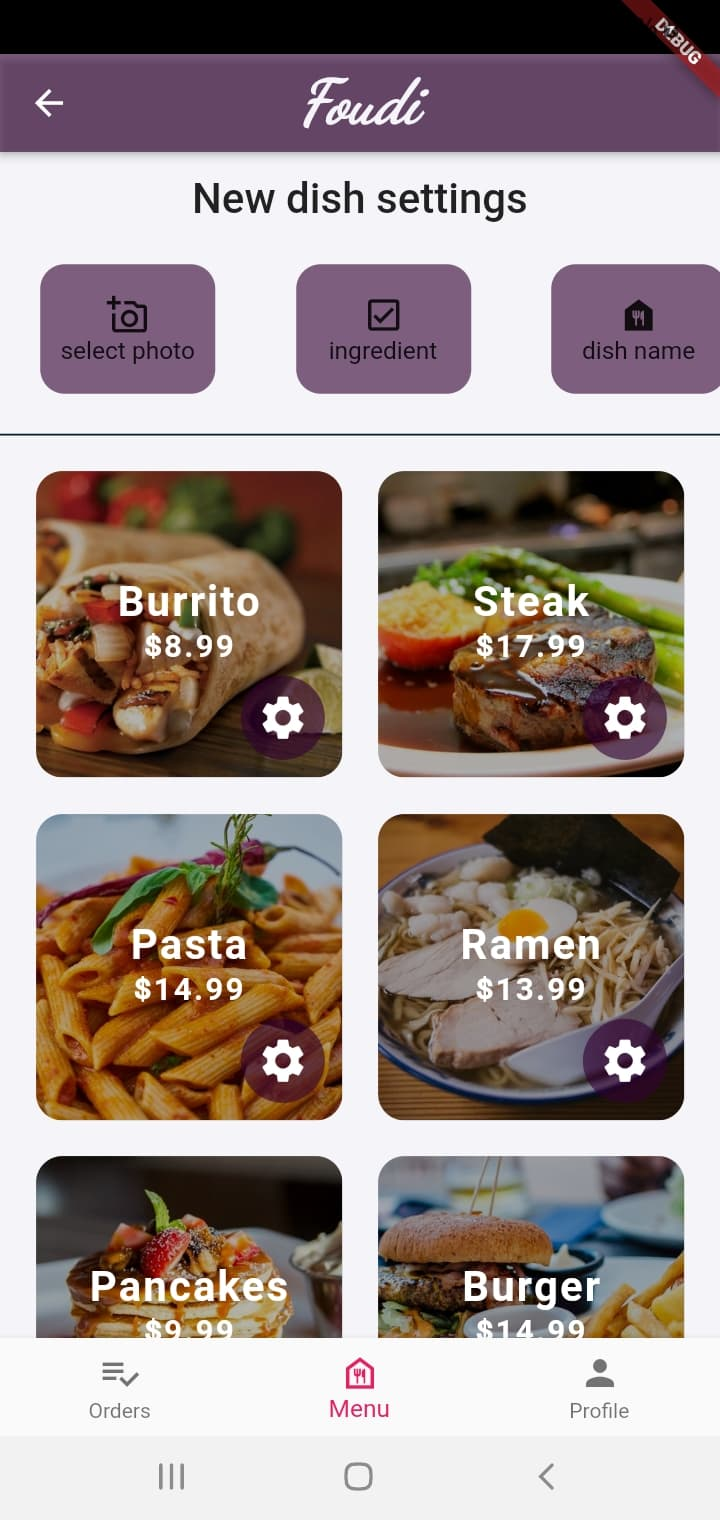
\includegraphics[width=.9\linewidth]{screenshots/Restaurantviews/MenuSetup.jpg}
  \caption{L'IHM du menu}
  \label{fig:restconfig}
\end{subfigure}%
\begin{subfigure}{.5\textwidth}
  \centering
  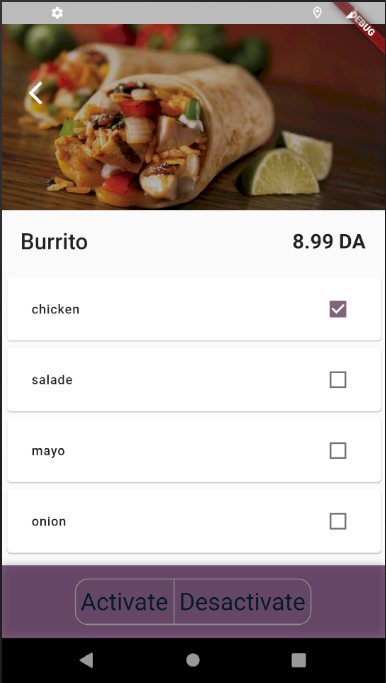
\includegraphics[width=.9\linewidth]{screenshots/Restaurantviews/ModifyDish.png}
  \caption{L'IHM de la page de modification d'un plat}
  \label{fig:restedit}
\end{subfigure}
\caption{Le IHMs de configuration de menu}
\label{fig:restmnu}
\end{figure}
		
	\subsection{Page de profile} Lorsque le restaurant fait l'objet d'une critique de la part de ses clients, lorsque l'employé du restaurant consulte son profil, il peut voir toutes les critiques et tous les commentaires (fig \ref{fig:restprof}).
	
	\begin{figure}[h!]
			\center
			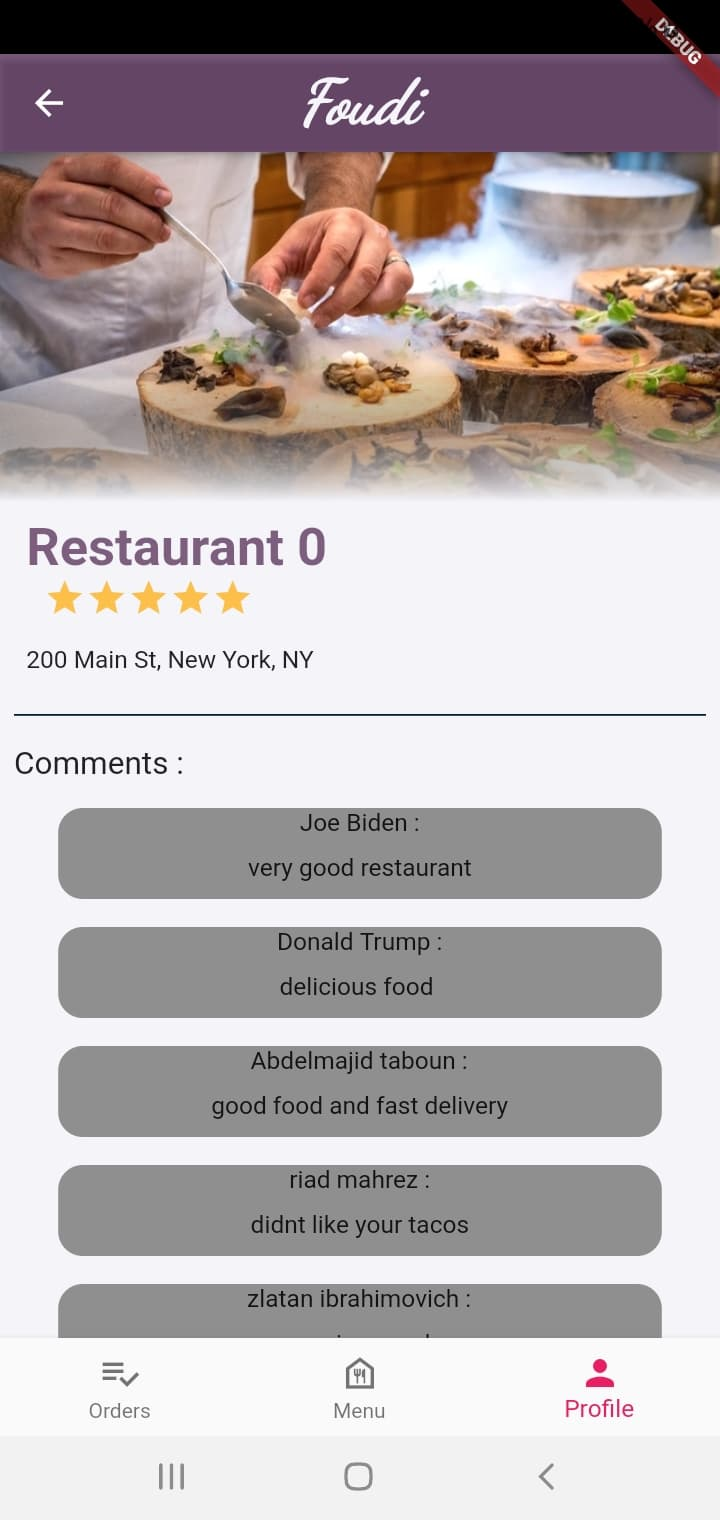
\includegraphics[width=5cm]{screenshots/Restaurantviews/ProfileWithReviews.jpg}
			\caption{L'IHM de la page de profile de restaurant}
			\label{fig:restprof}	
		\end{figure}
		
		
	\newpage
	\section{Cas d'utilisateur livreur} Le livreur dispose de trois pages dans le menu de l'application:
		\begin{itemize}
			\item \textbf{Page d'accueil}: Affiche les livraisons à proximité
			\item \textbf{Page des statistiques}: Montre quelques chiffres sur toutes ses livraisons et la progression des livraisons dans le temps,
			\item \textbf{Page de profile}: Pour voir son rating, et changer les détails de son compte.
		\end{itemize}
	
		\subsection{La page d'accueil} 
		\begin{figure}[h!]
			\center
			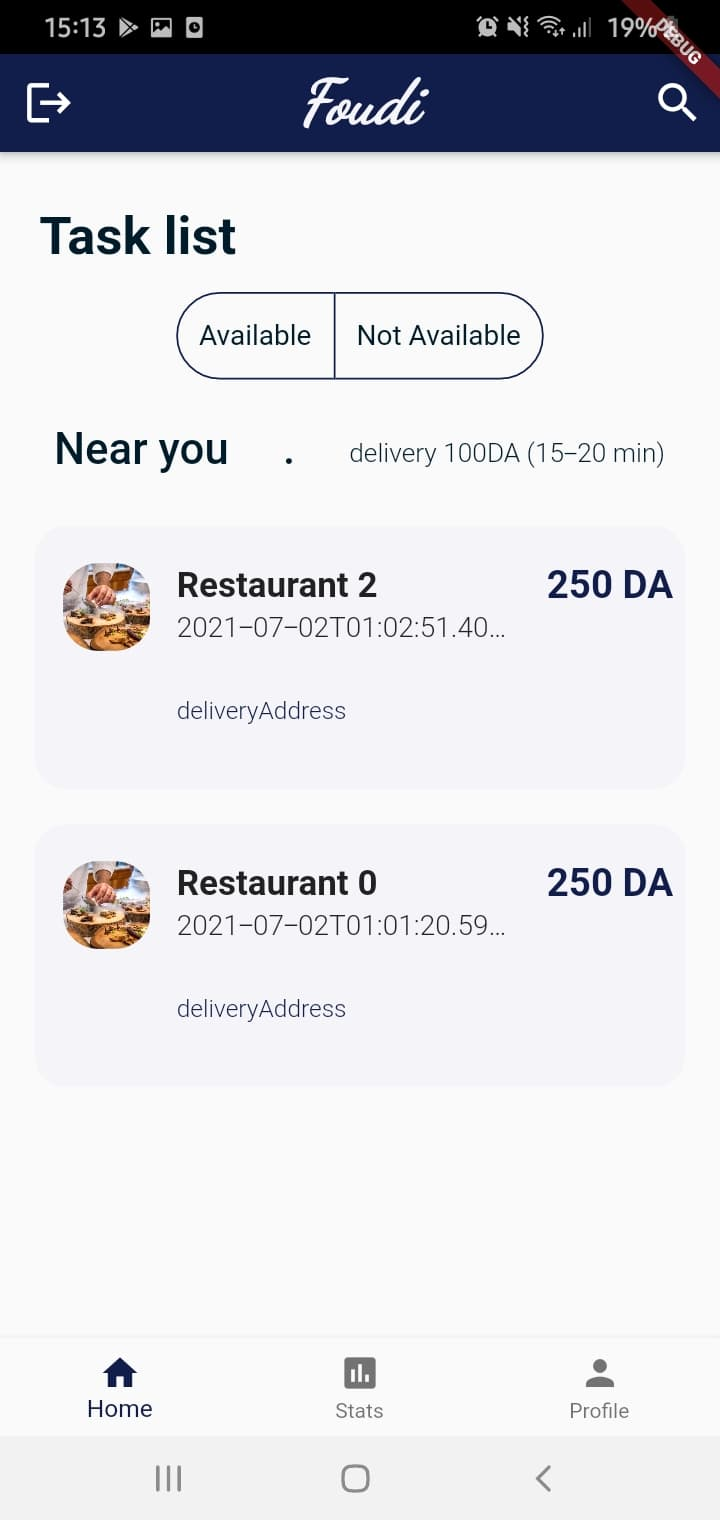
\includegraphics[width=5cm]{screenshots/DeliveryViews/Homepage(list of orders).jpg}
			\caption{L'IHM de la page d'accueil du livreur}
			\label{fig:delihp}
		\end{figure}
		La page d'accueil du livreur (fig \ref{fig:delihp}) est constituée des commandes proches prêtes à être livrées ; la liste des commandes contient les informations essentielles de chaque commande qui permettent à l'utilisateur de la choisir ou de l'ignorer.
		\newpage
		\begin{figure}[h!]
			\center
			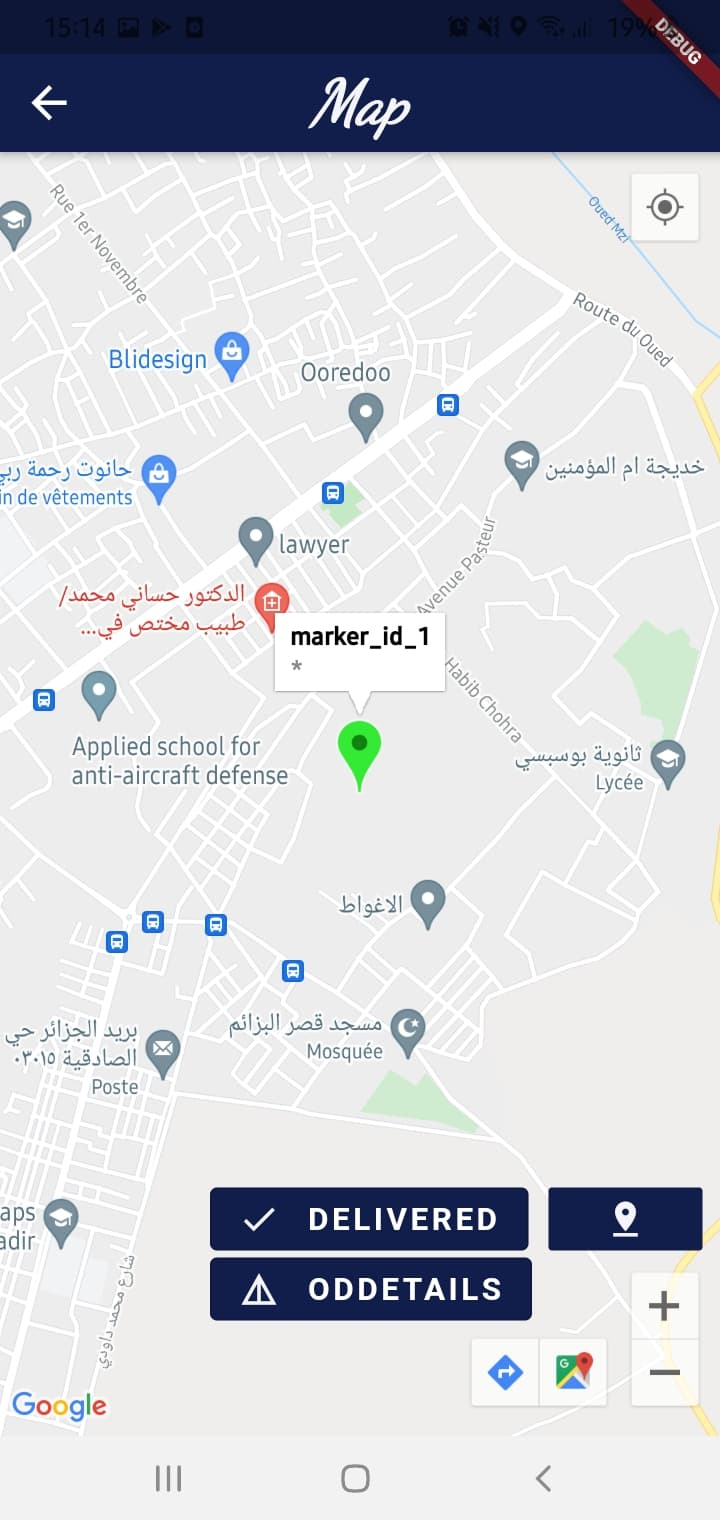
\includegraphics[width=5cm]{screenshots/DeliveryViews/ClientPositionMap.jpg}
			\caption{L'IHM de la carte de livreur}
			\label{fig:delimp}
		\end{figure}
		
		Lorsqu'il sélectionne une commande à livrer, l'application affiche la carte avec les emplacements du restaurant et du client (fig \ref{fig:delimp}).
Une fois qu'il a livré la commande, il peut appuyer sur le bouton "livré" indiqué sur la carte.

\newpage
\chapter*{Conclusion}
Notre application n'est pas destinée à fonctionner avec un seul restaurant ou établissement de livraison, nous avons créé une plateforme qui regroupe tous les différents établissements pour travailler en un seul endroit.\\


Notre principal objectif en créant l'application n'était pas seulement d'apprendre à la concevoir ou d'acquérir l'expérience du développement d'une grande application mobile, mais de l'utiliser comme notre entrée dans le monde des affaires et de conquérire avec cette application le marché algérien en ligne.\\


Pour l'instant, l'application fonctionne à petite échelle, nous nous préparions à ajouter de nombreuses caractéristiques et fonctionnalités pratiques, mais en raison du peu de temps qui nous a été accordé, nous n'avons pas atteint le produit souhaité.\\


Nous allons continuer à développer cette idée et la pousser à l'extrême car nous avons remarqué que nous offrons en général une solution moins chère et plus efficace.

\addcontentsline{toc}{chapter}{Conclusion}

\newpage
\begin{thebibliography}{300}
\end{thebibliography}

\end{document}
